%%%%%%%%%%%%%%%%%%%%%%%%%%%%%%%%%%%%%%%%%
% Large Colored Title Article
% LaTeX Template
% Version 1.1 (25/11/12)
%
% This template has been downloaded from:
% http://www.LaTeXTemplates.com
%
% Original author:
% Frits Wenneker (http://www.howtotex.com)
%
% License:
% CC BY-NC-SA 3.0 (http://creativecommons.org/licenses/by-nc-sa/3.0/)
%
%%%%%%%%%%%%%%%%%%%%%%%%%%%%%%%%%%%%%%%%%

%----------------------------------------------------------------------------------------
%	PACKAGES AND OTHER DOCUMENT CONFIGURATIONS
%----------------------------------------------------------------------------------------

\documentclass[DIV=calc, paper=a4, fontsize=11pt, twocolumn]{scrartcl}	 % A4 paper and 11pt font size

\usepackage{lipsum} % Used for inserting dummy 'Lorem ipsum' text into the template
\usepackage[english]{babel} % English language/hyphenation
\usepackage[protrusion=true,expansion=true]{microtype} % Better typography
\usepackage{amsmath,amsfonts,amsthm} % Math packages
\usepackage[svgnames]{xcolor} % Enabling colors by their 'svgnames'
\usepackage[hang, small,labelfont=bf,up,textfont=it,up]{caption} % Custom captions under/above floats in tables or figures
\usepackage{booktabs} % Horizontal rules in tables
\usepackage{fix-cm}	 % Custom font sizes - used for the initial letter in the document

\usepackage{sectsty} % Enables custom section titles
\allsectionsfont{\usefont{OT1}{phv}{b}{n}} % Change the font of all section commands

\usepackage{fancyhdr} % Needed to define custom headers/footers
\pagestyle{fancy} % Enables the custom headers/footers
\usepackage{lastpage} % Used to determine the number of pages in the document (for "Page X of Total")

% Headers - all currently empty
\lhead{}
\chead{}
\rhead{}

% Footers
\lfoot{}
\cfoot{}
\rfoot{\footnotesize Page \thepage\ of \pageref{LastPage}} % "Page 1 of 2"

\renewcommand{\headrulewidth}{0.0pt} % No header rule
\renewcommand{\footrulewidth}{0.4pt} % Thin footer rule

\usepackage{lettrine} % Package to accentuate the first letter of the text
\newcommand{\initial}[1]{ % Defines the command and style for the first letter
\lettrine[lines=3,lhang=0.3,nindent=0em]{
\color{DarkGoldenrod}
{\textsf{#1}}}{}}

%----------------------------------------------------------------------------------------
%	TITLE SECTION
%----------------------------------------------------------------------------------------

\usepackage{titling} % Allows custom title configuration

\newcommand{\HorRule}{\color{DarkGoldenrod} \rule{\linewidth}{1pt}} % Defines the gold horizontal rule around the title

\pretitle{\vspace{-30pt} \begin{flushleft} \HorRule \fontsize{50}{50} \usefont{OT1}{phv}{b}{n} \color{DarkRed} \selectfont} % Horizontal rule before the title

\title{Article Title} % Your article title

\posttitle{\par\end{flushleft}\vskip 0.5em} % Whitespace under the title

\preauthor{\begin{flushleft}\large \lineskip 0.5em \usefont{OT1}{phv}{b}{sl} \color{DarkRed}} % Author font configuration

\author{John Smith, } % Your name

\postauthor{\footnotesize \usefont{OT1}{phv}{m}{sl} \color{Black} % Configuration for the institution name
University of California % Your institution

\par\end{flushleft}\HorRule} % Horizontal rule after the title

\date{} % Add a date here if you would like one to appear underneath the title block

%----------------------------------------------------------------------------------------
%	SECTION TITLE
%----------------------------------------------------------------------------------------

%\usepackage{titlesec}

%\titleformat{\section}{\normalfont\scshape}{\thesection}{1em}{}

%\titleformat{\subsection}{\normalfont\scshape}{\thesection}{1em}{}

%----------------------------------------------------------------------------------------

\begin{document}

\maketitle % Print the title

\thispagestyle{fancy} % Enabling the custom headers/footers for the first page 

%----------------------------------------------------------------------------------------
%	ABSTRACT
%----------------------------------------------------------------------------------------

% The first character should be within \initial{}
\initial{H}\textbf{ere is some sample text to show the initial in the introductory paragraph of this template article. The color and lineheight of the initial can be modified in the preamble of this document.}

%----------------------------------------------------------------------------------------
%	ARTICLE CONTENTS
%----------------------------------------------------------------------------------------

\section*{Introduction}

\subsection*{What is curiosity?}
\initial{B}efore we begin, it is relevant to take a moment to fully digest the course of human history, and where we are now.
We started humble.
From our beginnings as hunter-gatherers in a nomad lifestyle with no more tools than those fashioned from stone, and no sharing of knowledge save amongst the tribal units.
Given a few thousand years, we have gone from looking at the stars with wonder to looking at the stars with determination.
The human race has reached a stage where we are capable of putting human beings into metal boxes propelled by tiny explosions and launching them out of our atmosphere.
All of this has, at some point, existed as an idea in the mind of a curious human being.
The discoveries in biology that have given us insights into how we are constructed, and the progresses of physics and engineering that have allowed us to build spacefaring crafts; all has at some point only been a figment of someone's imagination.

When the Russian cosmonauts first escaped our planet's gravity, a new realm of potential discoveries were released.
The imagination has been exposed to an embarrassment of riches since then.
The curious human mind, having discovered that the universe is vast and open to our travel, and that the unique conditions of temperature, pressure and matter that have made \textit{us}, likely exist elsewhere in the universe:

Can we reach other worlds?
What will we find there?
\textit{Are we alone?}
The thrill of discovery is immense.
Understanding history as we do, we know that a large number of years have passed, a large number of discoveries have been made, and many wise lives have come and gone and contributed to the ladder of knowledge we are currently climbing.
To fully understand our current hunt for extra-terrestrial life we need a context and to fully respect it, we must know who contributed, and how.

%------------------------------------------------

\section*{The history of astronomy and biology}

\subsection{Egyptians: Astronomy as a tool for agriculture and belief}
\initial{S}ome celestial bodies like the Sun and the Moon were documented already five thousand years ago!
Indeed, astronomy being a science of observation, Egyptians did not need more than looking into the sky to discover bodies.
Although more difficult to observe, five planets could already be seen by the naked eye due to their size and brightness:
Mercury, Venus, Jupiter, Mars and Saturn.
However, we had to wait until Copernicus in 1543 to finally recognize Mars as a planet!

Egyptians' main interests for the sky were mainly agricultural and religious.
The Egyptians studied the positions and alignments of stars to build pyramids, and the size of the Moon determined periods of harvest.
For the same purpose, they already used the 365 days calendar.
Religion also played a great part in ancient astronomy as gods were viewed as constellations.
\cite{Egyptians}

\begin{center}
	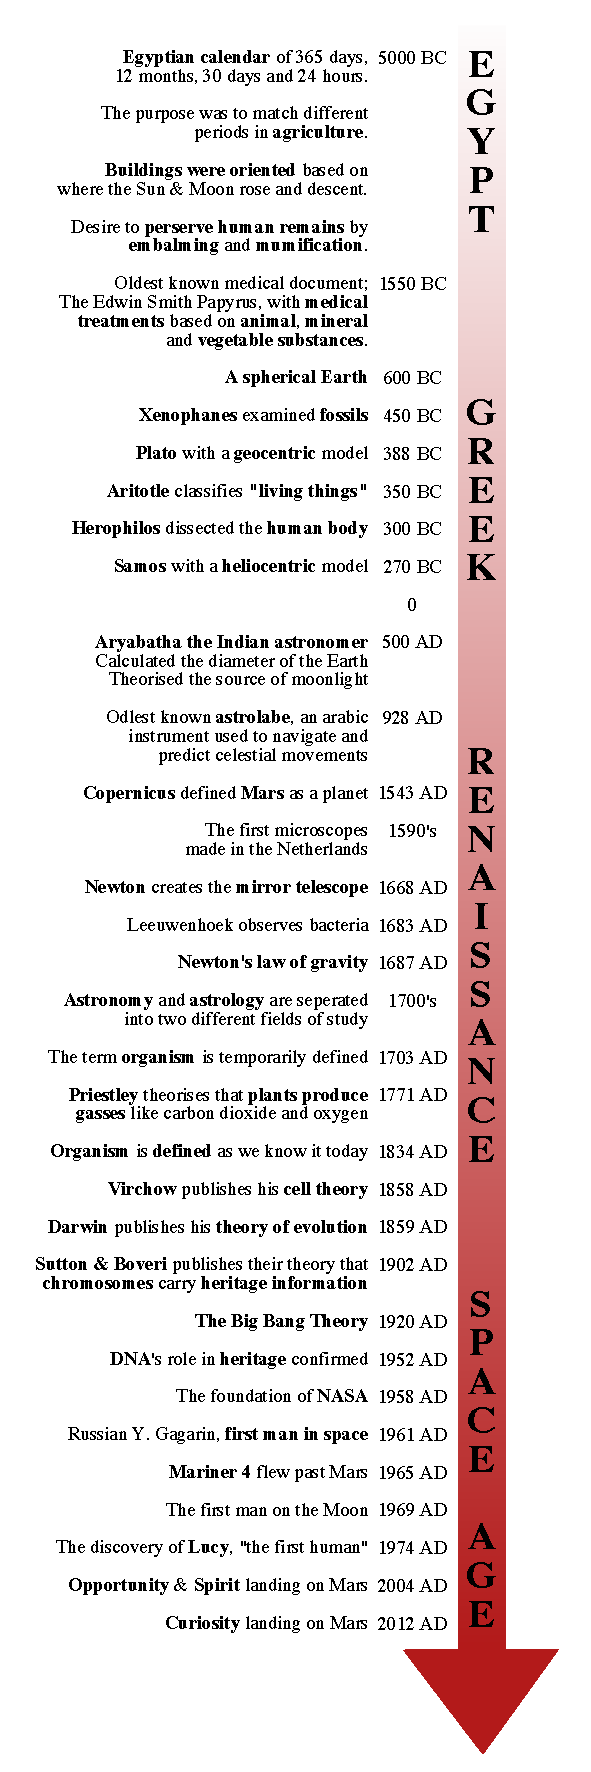
\includegraphics[width=0.475\textwidth]{timeline.pdf}
\end{center}

\subsection{Ancient Greeks, Arabs and Indians: The age of theories}
\initial{I}t is not until the Greek period, starting around 600 BC, that humanity tried to really understand and explain astronomy. 
To start with, they thought that Earth was flat, surrounded by water and that the stars were emerging from it.
Plato, followed by Ptolemy and Aristotle, were the pioneers of the geocentric model: the Sun, the Moon and the planets move in harmony around Earth, the center.

A hundred years later, another Greek, Samos, proposed the opposite theory called heliocentrism: the Sun is now the center of the Universe.
How fascinating to see how much they actually discovered at that time!  
Without tools such as the telescope, without communication within the community of scientists around the world, Greeks, Arabs and Indians still made great assumptions on how our universe worked. 
For example, the Indian astronomer, Aryabatha, not noly did he have some ideas about gravitation but also that the movement of planets around the Sun were elliptical and not circular.
He even understood that the light coming from the Moon was refracted sunlight, and not the Moon itself glowing in the dark sky.
One might wonder, how much we would know in the present time if ancient astronomers had the tools of communication we have today?
\cite{GreekAstro}
\cite{Aryabatha}

\subsection{European Renaissance: The age of reason and experimentation}
\initial{W}ith new technologies and the rediscoveries and translations of ancient Greek texts, the scientists of the renaissance period, were able to make very accurate calculations of the stars and planets.
Intellectuals in this period defined and proved the basic of astronomy as we know it today.  
Scientists such as Copernicus, Galileo and Kepler defined the heliocentric model to the world. 
It was definitely the age of reason and scientific truth. 
We can notice for example, that it is during that time that astronomy and astrology were separated into two different fields. 
Technologies and communications became more advanced and enabled physicists to search deeper and with more accuracy. 
In 1609, the Italian astronomer Galileo was one of the first people to point a telescope skyward. 
Although that telescope was far from perfected, Galileo was able to see that the Moon's surface was made of craters and mountains instead of being smooth as we thought.
As their view expanded dramatically by the telescope, astronomers were also able to discover many stars and to calculate stellar distances.
\cite{GalileoTelescope}

\subsection{Space Age: Not only studying Astronomy but also Exploring!}
\initial{I}n 1957, The Soviet Union launched Sputnik, the first spacecraft placed in orbit around Earth, marking the beginning of space exploration.
We are not only interested in studying, but also of exploring.
The space age represents an effort that is as scientific as it is political.
Indeed, this happened during the Cold War when the Soviet Union and the USA raced in different domains, including astronomy.

This space race focused particularly on discovery by humans and machines in the solar system and the development of technology.
Rockets were one of the most obvious forms of space age technology.
The creation of NASA, followed by the Apollo program was definitely highlights of the space age.
The most famous of the Apollo aircrafts was Apollo 11, carrying commander Neil Armstrong and his fellow astronauts Michael Collins and Edwin 'Buzz' Aldrin to the Moon.
On that mission, Armstrong and Aldrin were the first humans to land and walk on the Moon.
"That's one small step for a man, one giant leap for mankind."
\cite{SpaceAge}

\begin{tcolorbox}[colback=green!5,colframe=green!40!black,title=The wow! signal: Our first Extra-Terrestrial communication ? ]

On a night in 1977, Jerry Ehman, working for SETI (Search for Extra-Terrestrial Intelligence) took part in one of the world's biggest mysteries: The Wow! signal.

He was working on radio frequencies used as signals. The system is simple:\\

We measure intensity of radio frequencies. The intensity goes from 0 (the lowest) to 35 (the highest).  The intensity of the signal is normally between 0 and 2. But for 72 seconds he got an extraordinary signal: 6EQUJ5 from non-solar origin. A signal that was at its highest (the letter U) 30 times greater than the ordinary deep space noise! Amazed, Ehman wrote on the side: "Wow!", which simply became the name of the signal. But despite different theories and research on this signal, we still have no clue on what happened that night in 1977... \\

\textbf{What is 6EQUJ5?} \\

The intensity is measured between 0 and 35. Instead of just using numbers we changed 0 into a space and each numbers after 9 with the corresponding letter of the English alphabet. For example Q= 26 and U=30 

%------------------------------------------------

\section*{Physics crash course}

\subsection*{Entropy}
Imagine a room full of balls bouncing off the walls and each other.
Your image is probably a chaotic mess of balls traveling in all directions and speeds.
The order, or disorder, of the balls is what physicists call entropy.

Entropy is derived from thermodynamics, and it explains some of the most fundamental laws of our universe.

To understand what entropy really means, imagine all of the bouncing balls in your room being in the same corner at the same time.
This must be a very unlikely occurrence.
There are few ways to place all of the balls together in one corner, but lots of ways to spread them all around the room.
When all the balls are in the corner, the room has a low entropy.
If the balls are all over the place, the entropy is high.


The second law of thermodynamics says that the entropy in a closed system never decrease.
In other words; no matter what happens in a closed system, for example a room with no interaction with the outside world, there will be more and more chaos over time.
The system, or room, will eventually reach what we call a thermodynamic equilibrium.
If you want to keep the order in you room, you will need to supply it with energy.
That is partially why humans needs to eat.
Our cells use energy in chemical reactions, and we need to keep the entropy low in order for these chemical reactions to continue.
That is living beings has to be able to work against an increase in entropy, and also the reason this is one of the requirements we use to define life as we know it.

\subsection*{Spectroscopy, radiation and nuclear physics}








Spectroscopy is a method used in experimental physics to obtain information about a material.
In general one sends some kind of radiation towards the material, and then observes what happens afterwards.
Common radiation used in spectroscopy is photons, alpha, beta and gamma radiation.



% Diffraction

%----------------------------------------------------------------------------------------
%	REFERENCE LIST
%----------------------------------------------------------------------------------------

\begin{thebibliography}{99} % Bibliography - this is intentionally simple in this template

\bibitem[Figueredo and Wolf, 2009]{Figueredo:2009dg}
Figueredo, A.~J. and Wolf, P. S.~A. (2009).
\newblock Assortative pairing and life history strategy - a cross-cultural
  study.
\newblock {\em Human Nature}, 20:317--330.
 
\end{thebibliography}

%----------------------------------------------------------------------------------------

\end{document}